\documentclass[a4paper]{article}

%%%%%%%% CREATE DOCUMENT STRUCTURE %%%%%%%%
%% Language and font encodings
\usepackage[english]{babel}
\usepackage[utf8x]{inputenc}
\usepackage[T1]{fontenc}
%\usepackage{subfig}

%% Sets page size and margins
\usepackage[a4paper,top=3cm,bottom=2cm,left=2cm,right=2cm,marginparwidth=1.75cm]{geometry}

%% Useful packages
\usepackage{amsmath,amssymb}
\usepackage{graphicx}
\usepackage[colorinlistoftodos]{todonotes}
\usepackage[colorlinks=true, allcolors=blue]{hyperref}
\usepackage{caption}
\usepackage{subcaption}
\usepackage{sectsty}
\usepackage{apacite}
\usepackage{float}
\usepackage{titling} 
\usepackage{blindtext}
\usepackage[square,sort,comma,numbers]{natbib}
\usepackage[colorinlistoftodos]{todonotes}
\usepackage{xcolor}
\definecolor{darkgreen}{rgb}{0.0, 0.4, 0.0}
\usepackage{graphicx}
\newcommand{\norm}[1]{\left\lVert#1\right\rVert}
\DeclareMathOperator{\R}{\mathbb{R}}
\DeclareMathOperator{\E}{\mathbb{E}}

\usepackage{listings}
\usepackage{xcolor}

\definecolor{codegreen}{rgb}{0,0.6,0}
\definecolor{codegray}{rgb}{0.5,0.5,0.5}
\definecolor{codepurple}{rgb}{0.58,0,0.82}
\definecolor{backcolour}{rgb}{0.95,0.95,0.92}

\lstdefinestyle{mystyle}{
	backgroundcolor=\color{backcolour},   
	commentstyle=\color{codegreen},
	keywordstyle=\color{magenta},
	numberstyle=\tiny\color{codegray},
	stringstyle=\color{codepurple},
	basicstyle=\ttfamily\footnotesize,
	breakatwhitespace=false,         
	breaklines=true,                 
	captionpos=b,                    
	keepspaces=true,                 
	numbers=left,                    
	numbersep=5pt,                  
	showspaces=false,                
	showstringspaces=false,
	showtabs=false,                  
	tabsize=2
}

\lstset{style=mystyle}
 



%%%%%%%% DOCUMENT %%%%%%%%
\begin{document}

%%%% Title Page
\begin{titlepage}

\newcommand{\HRule}{\rule{\linewidth}{0.5mm}} 							% horizontal line and its thickness
\center 
 
 
% University


\includegraphics[width=0.15\textwidth]{images/kth_logo.png}\\[0.5cm] 	% University logo

\textsc{\LARGE KTH Royal Institute of Technology}\\[1cm]

% Document info
\textsc{\Large Deep Learning in Datascience}\\[0.2cm]
\textsc{\large DD2424}\\[1cm] 										% Course Code
\HRule \\[0.8cm]
{ \huge \bfseries Assignment 1 (Bonus)}\\[0.7cm]								% Assignment
\HRule \\[2cm]
\large
\emph{Authors:}\\
Ali Banaei Mobarak Abadi\\[1.5cm]													% Author info
{\large \today}\\[5cm]

\vfill 
\end{titlepage}

%%\begin{abstract}
%%Your abstract.
%%\end{abstract}

%%%% SECTIONS
%% Section 1
\section*{Question 2.1}
In this question we try to improve our network's peformance. To do so, we used the following methods.

\subsection*{Increasing training set}
As the fitst experiment, the size of the validation set was reduced to only 1K samples so we would have a bigger training set. We then trained the model with four different settings as before. The results of evaluation on test set are presented in \autoref{tab:bigger_training}.

\begin{table}[h]
	\centering
	\caption{Evaluation of the model trained on bigger training set.}
	\label{tab:bigger_training}
	\begin{tabular}{|l|l|l|l|l|}
		\hline
		$\lambda$ & $\eta$ & Loss & Cost & Accuracy \\ \hline
		0         & 0.1    & 6.70 & 6.70 & 0.26     \\ \hline
		0         & 0.001  & 2.01 & 2.01 & 0.33     \\ \hline
		0.1       & 0.001  & 1.74 & 1.79 & 0.40     \\ \hline
		1         & 0.001  & 1.85 & 1.92 & 0.37     \\ \hline
	\end{tabular}
\end{table}

Now, if we compare these values and ones we got in the last part, we do not see any significant changes (for more confident conclusion, we may need to perform multiple tests and use significance tests, but here based on our inductive expectation and the values we can be sure the difference is not significant). It was expected that this will not lead to a major enhancement since the number of samples was not a major concern for us (we had enough samples to train our simple model).

\subsection*{Augmenting the trainig data}

In this part, the effect of augmentation was investigated. In each step, in order to make a minibatch, we perform flipping by the probability of 0.5 for each sample. As we saw, despite some minor increases in performance in some cases, this method does not have a huge impact. One may again use the same argument that before which since we have a considerable amount of data and a very simple network, these methods, which aim to increase the diversity of the input data fed to the network, may not have a significant impact since the bottleneck here is the low complexity of the model. The test results for this part can be found in \autoref{tab:flipping}.

\begin{table}[h]
	\centering
	\caption{Performance of trained network using data agumentation on test data}
	\label{tab:flipping}
	\begin{tabular}{|l|l|l|l|l|}
		\hline
		$\lambda$ & $\eta$ & Loss & Cost & Accuracy \\ \hline
		0         & 0.1    & 5.91 & 5.91 & 0.30     \\ \hline
		0         & 0.001  & 2.02 & 2.02 & 0.33     \\ \hline
		0.1       & 0.001  & 1.74 & 1.80 & 0.41     \\ \hline
		1         & 0.001  & 1.85 & 1.92 & 0.38     \\ \hline
	\end{tabular}
\end{table}


\subsection*{Learning rate decay}

As the next improvement method, learning rate decay was used. At the beginning of the learning process, the learning rate was set to 0.01. Then, after 20 epochs, it was changed to 0.001. Then, after every 40 epochs, the learning rate was divided by 10. Increasing the learning rate after we converge to a flat area may help the network to converge faster to the optimal values instead of keeping jumping around it. As we can see in \autoref{fig:schedule}, on epochs that we decrease the learning rate, we have a sudden increase in accuracy and decrease in the loss function. Also, the performance of the network on the test data was increased, and in the end, we reached an accuracy of almost 0.43, which we had never seen before.

\begin{figure}[h]
	\centering
	\begin{subfigure}{\textwidth}
		\centering
		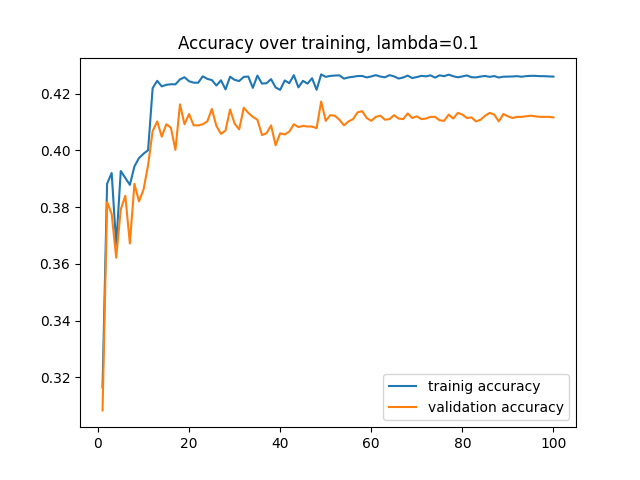
\includegraphics[width=.6\linewidth]{images/scheduled_accuracy_over_trainig_lambda=0.1.png}
	\caption{Accuracy}
	\end{subfigure}
	\begin{subfigure}{\textwidth}
		\centering
		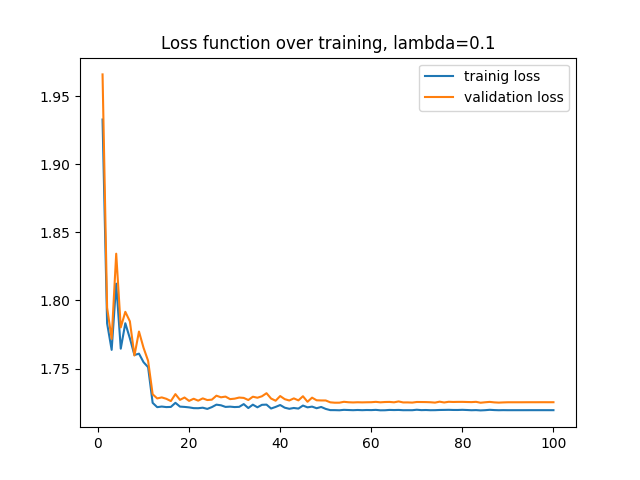
\includegraphics[width=.6\linewidth]{images/scheduled_loss_over_trainig_lambda=0.1.png}
		\caption{Loss value}
	\end{subfigure}

	\caption{Loss and accuracy on training and validation data during trainig using a learning rate scheduler.}
	\label{fig:schedule}
\end{figure}



\section*{Question 2.2}
We first derive the partial derivative of the loss function with respect to $p_k$. 

\begin{align*}
	& \frac{\partial l}{\partial p_k} = \frac{\partial \big( -\frac{1}{K}[(1-y_k) \log(1-p_k) + y_k \log(p_k)]\big)}{\partial p_k} = -\frac{1}{K} [ (1-y_k) \frac{-1}{1-p_k} + y_k \frac{1}{p_k}] = \\
	& - \frac{1}{K} [\frac{y_k - 1}{1 - p_k} + \frac{y_k}{p_k}] = -\frac{1}{K} \frac{y_k - p_k}{p_k (1-p_k)}
\end{align*}

Now, we have

\begin{align*}
	& \frac{\partial p_k}{s_k} = \frac{\partial}{\partial s} (1 + e^{-s_k})^{-1} = -1 (1 + e^{-s_k})^{-2} (-e^{-s_k}) = \frac{1}{1 + e^{-s_k}} \frac{e^{-s_k}}{1 + e^{-s_k}} = \\
	& \frac{1}{1 + e^{-s_k}}  \big( 1 -  \frac{1}{1 + e^{-s_k}} \big) = \sigma(s_k) (1-\sigma(s_k)) = p_k (1-p_k)
\end{align*}


And finally we have

$$
	\frac{\partial l}{\partial s_k} = \frac{\partial l}{\partial p_k} \frac{\partial p_k}{\partial s_k} = \frac{1}{K} \frac{p_k - y_k}{p_k (1-p_k)} p_k (1-p_k) = \frac{1}{K} (p_k - y_k)
$$

So, as we see, this is the same as cross-entropy with softmax activation except the devision by the number of classes. So, in the code we only need to change the forward pass (replacing the softmax with sigmoid) and in gradient descent we can simply devide the gradients by the number of classes. Since all the trainable parameters are before $s$ then this method will result in the same learning.


After training the network with the new objective function, the model was evaluated on the test results. The new model reached the accuracy of 0.33 while the former model could reach 0.32 when we used $\eta_{CE}=0.001, \eta_{MBCE}=0.01, \lambda=0$. As we see, the two models perform very closely. [] shows the histogram of probabilities for both models. The histograms are very similar to each other, although in multiple binary classification methods, we have some winner classes that have a probability below 0.2. In cross-entropy, since we use softmax and all probabilities sum to one, then we do not see a lot of winner classes with low assigned probability. But because in the M-BCE, we do not have this constraint, the probability of winner classes is more freely set.
Also, [] depicts the validation and training set loss during training. As we see, the cross-entropy method shows a gap between training and validation loss, while the two curves are almost identical in M-BCE. So, the M-BCE is less prone to overfitting.


\begin{figure}[h]
	\centering
	\begin{subfigure}{\textwidth}
		\centering
		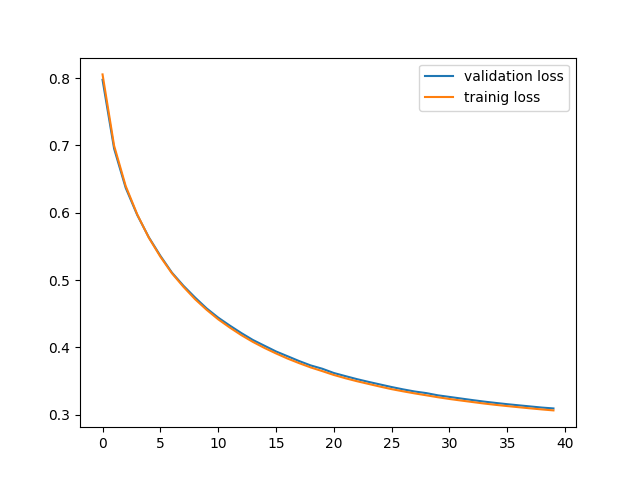
\includegraphics[width=.6\linewidth]{images/mbce_loss.png}
		\caption{Multiple-BCE}
	\end{subfigure}
	\begin{subfigure}{\textwidth}
		\centering
		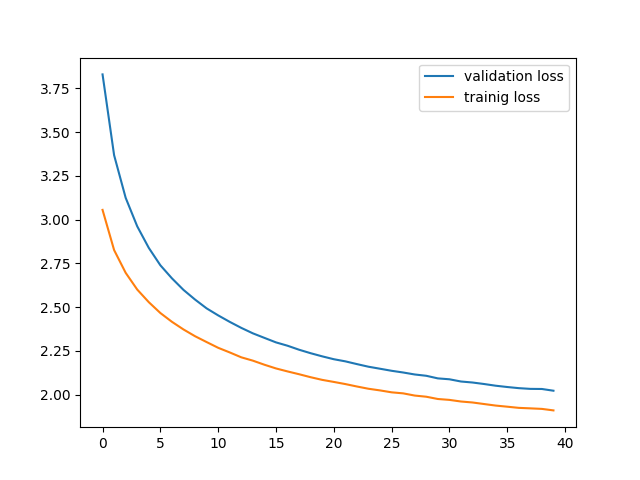
\includegraphics[width=.6\linewidth]{images/simple_loss.png}
		\caption{Cross-validation}
	\end{subfigure}
	
	\caption{Loss on training and validation data during trainig.}
	\label{fig:mbce_loss}
\end{figure}


\begin{figure}[h]
	\centering
	\begin{subfigure}{\textwidth}
		\centering
		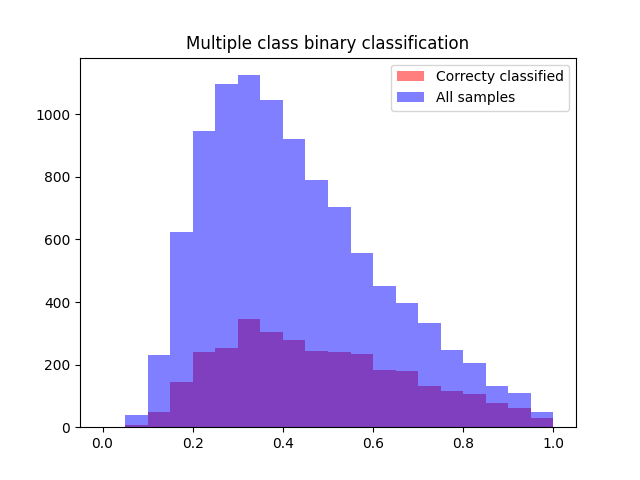
\includegraphics[width=.6\linewidth]{images/mbce_lamb0.png}
		\caption{Multiple-BCE}
	\end{subfigure}
	\begin{subfigure}{\textwidth}
		\centering
		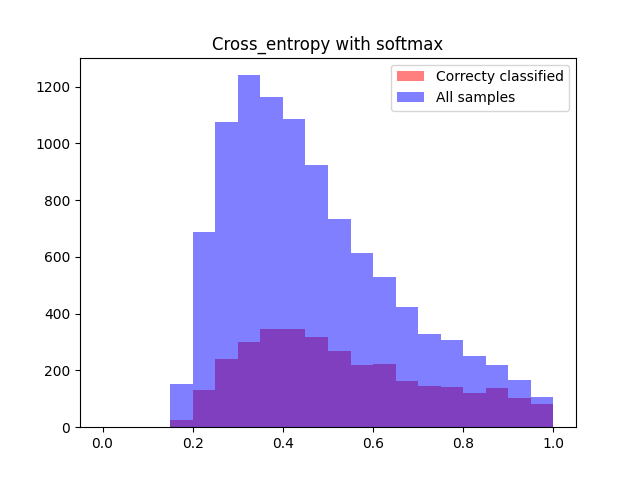
\includegraphics[width=.6\linewidth]{images/simple_lamda0.png}
		\caption{Cross-entropy}
	\end{subfigure}
	
	\caption{Histogram of the true class probabilities.}
	\label{fig:mbce_hist}
\end{figure}


\section*{Code documentation}
Please go to the report for the mandatory part of the assignment for a full explanation of the implementation.


%%%%%%%% EXTRA TIPS %%%%%%%%
%% If you want to include an figure
%%\begin{figure}[H]
%%\includegraphics[]{Pendulum.jpg}
%%\caption{Sketch of the pendulum}
%%\label{fig:pendulum}
%%\end{figure}

%% for multiple figures in one fig
%\begin{figure}[h]
%	\centering
%	\begin{subfigure}{\textwidth}
%		\centering
%		\includegraphics[width=\linewidth]{images/sthfivo.png}
%		\caption{}
%	\end{subfigure}
%	\begin{subfigure}{\textwidth}
%		\centering
%		\includegraphics[width=\linewidth]{images/sth.png}
%		\caption{}
%	\end{subfigure}
%	\begin{subfigure}{\textwidth}
%		\centering
%		\includegraphics[width=\linewidth]{images/sth.png}
%		\caption{}
%	\end{subfigure}
%	\caption{caption}
%	\label{fig:label}
%\end{figure}


%% You can then reference with \ref{fig:pendulum}


%%\newpage


\end{document}